
\documentclass[a4paper]{article}

%% Language and font encodings
\usepackage[english]{babel}
\usepackage[utf8x]{inputenc}
\usepackage[T1]{fontenc}

%% Sets page size and margins
\usepackage[a4paper,top=2cm,bottom=2cm,left=3cm,right=3cm,marginparwidth=1.75cm]{geometry}

%% Useful packages
\usepackage{amsmath}
\usepackage{graphicx}
\usepackage[colorinlistoftodos]{todonotes}
\usepackage[colorlinks=true, allcolors=blue]{hyperref}

\providecommand{\keywords}[1]{\textbf{\textit{Tags:}} #1}
\providecommand{\talkurl}[1]{\textbf{\textit{Url:}} #1}
\providecommand{\track}[1]{\textbf{\textit{Track:}} #1}
\providecommand{\speaker}[1]{\textbf{\textit{Speaker:}} #1}



\title{'Horizon Zero Dawn' : A Game Design Postmortem \\by Eric Boltjes}
\author{Author: Bastien Pery}

\begin{document}
\maketitle

\begin{center}
  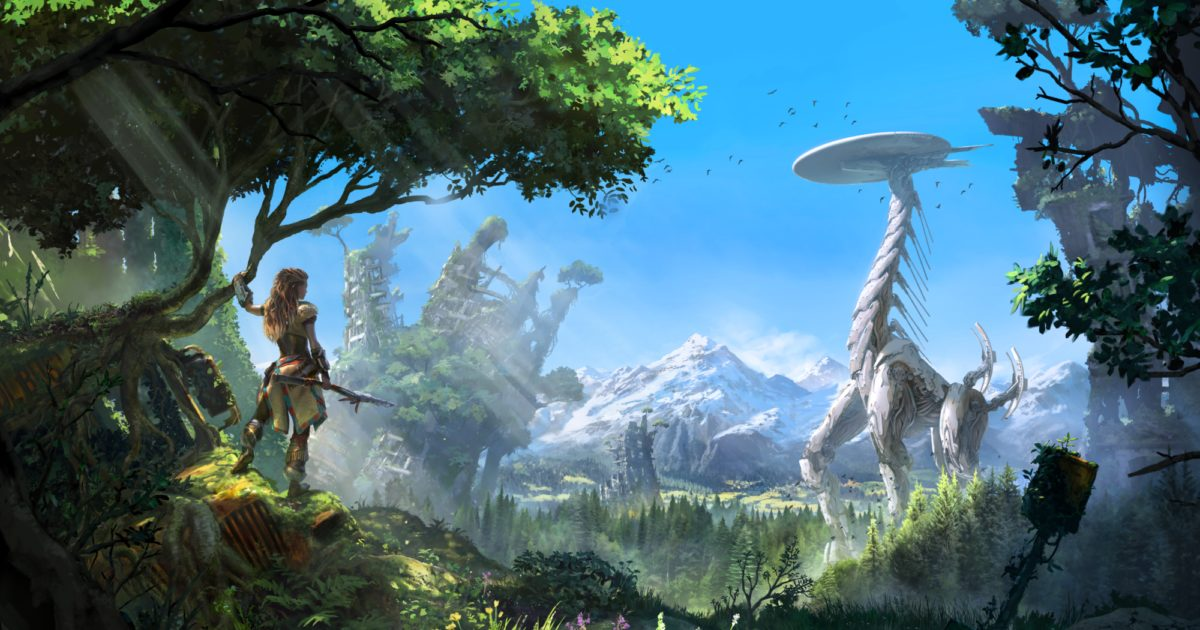
\includegraphics{Horizon.jpg}
\end{center}
\vspace{1em}

\begin{keywords} Horizon Zero Dawn, Game Design, Design decisions, Ambitious project \end{keywords}

\begin{track} GDC EXPO San Francisco March 2018 - Game Design \end{track}

\begin{talkurl}  \url{https://www.gdcvault.com/play/1024963/-Horizon-Zero-Dawn-A} \end{talkurl}

\begin{speaker}Eric Boltjes, Guerrilla Games \end{speaker}


\begin{abstract}
\end{abstract}

\section{Summary of Talk}

%%Your summary of the talk goes here! (in your own words!) 
%%Describe the main points / lessons learned of the talk, the relevance for game development. 

Through the creation of early prototypes and design decisions and processes that shaped
development of Horizon Zero Dawn, this talk takes us into the journey game design went through while 
moving from an ambitious paper concept to a finished open world action RPG. Thanks to Eric Boltjes'
details, this talk helps us to understand how small and large design decisions and choices can 
improve a game and players' experience.

\subsection{Early Concept}

Guerrilla Games studio never did an open world video game before. Here was for them the challenge
represented by Horizon. Indeed, the idea of the game came in 2001 with some important guidelines
such as :

\begin{itemize}
  \item Majestic post-apocalyptic wilderness
  \item Awe-inspiring machines (as an innovant concept)
  \item Exotic tribes
  \item And the open world idea 
\end{itemize}

\noindent But like all beginners, they didn't know how to structure that kind of game development. So,
they started with a really small team in 2011 composed by designers, artists, coders and 
animators. Each of them without a specific role. And, of course, with a lot of questions
(how the open world is going to look like, what kind of combat against machines we want and so on).\\

\noindent As they didn't have a global idea of how everything will work together, they decided to
do different prototypes to test them and judge their reliability. The feedbacks were very
good in the sense that these prototypes were really effective and helped them to know
what they wish to create for Horizon Zero Dawn. But it was costly in money and time. And also, 
prototype after prototype, the team started to think "Where is the game so?".\\

\noindent Thus, they answered two different fundamental questions before starting the pre-production:
\begin{itemize}
  \item What Horizon Zero Dawn is
  \item What it is NOT
\end{itemize}


\subsection{Pre-Production}

As they started to know where they were going, they focused on three major parts of the game for
the pre-production step:
\begin{itemize}
  \item World systems and mechanics
  \item World building
  \item Horizon Zero Dawn story
\end{itemize}

\noindent They so improved the size of the team by adding new responsabilities in it such as Core Design,
World Design, Story Design etc. Especially for the story, they didn't really thought about it
during the concept step. Everything still needed to be done.\\

\noindent They also worked to answer a lot of different questions they had. At this point, the team
still needed a context to be able to have the full game idea in their mind. So, they focused on
different parts of the game.
\begin{itemize}
  \item Riding (they wanted a special character so the normal horse has been replaced by a machine)
  \item The main character, Alloy (personality, style, gameplay...)
  \item Machines (behaviors, look and also "feelings")
\end{itemize}

\noindent Fixed contexts helped the team a lot. But be careful in game development, don't do it too 
soon or it will prevent cool ideas to come. Everything went well so they thought they had enough
answered to start the production in a good work environment. Unfortunately, problems started to appear.


\subsection{Production}

At the beginning of the production, Guerrilla's teams started to really show their lack of
knowledge in open world game development. Indeed, they faced quickly important problems in the game.\\

\noindent Firstly, they didn't know how to include efficiently a mechanics tutorial when the game starts.
Mostly because they didn't think about all the mechanics yet. Which is important to start every game
production.\\

\noindent Secondly, they also didn't go completely through the combat mechanics with machines.
They wanted a game accessible for everyone. Not too hard but also challenging. So they wanted
to give different ways to win a fight for the players through a bunch of weapons and abilities. Problem :
non experiment players will only use one type of weapon constantly. Thus, they add a way to see 
all machines' weaknesses to know instantly which weapon or combat tactical would be the best.\\

\noindent Thirdly, the human combat. It's quite challenging with the machines so it has to be
at least also a bit challenging with humans. Problem : fewer tactical options than with machines.
So they chose to use environment's elements to put the player more into the fights.\\

\noindent To summarize, Guerrilla underestimated the impact of encounter design and had to status about
problems which could have been resolved earlier. So every designer has to take care of every 
mechanics as soon as possible and don't rush into the production step.


\subsection{Polishment}

It's time to polish what they did. This step can be summarize in one sentence : playtesting a LOT. In 
this one it's possible (sure) that some new problems will appear. Horizon didn't
avoid it also. Indeed, because of all the different ressources the player can gather in the open world,
all the economy seemed to be quite difficult to understand. Every ennemy can give
a lot of various objects, specific for each race.\\

\noindent Unfortunately, Guerrilla didn't find a way to solve this problem and the
economy stayed quite complex to comprehend. So as game designer, find a key to have a simple
and accessible economy is also really important.


\subsection{Core points}

A game designer has to take care about everything and review all the points, all the time!
For examples, these are the most important points a game designer should be awared of:
\begin{itemize}
  \item Fix the goals (What do you want to achieve - be as clear as possible)
  \item Specify all the intentions you have for the game
  \item Be honnest with yourself (Don't be stubborn, if something doesn't work, it doesn't)
  \item Get ready for problems (Be flexible in everything to face problems easier and adapt yourself)
\end{itemize}

\section{Overview and Relevance}
%%Research on the topic of the talk; overall overview and the relevance of the 
%%technologies/techniques; give a short overview on the state of the art of the topic,
%% reference further readings and current developments. 

%%Provide a list of further readings, links (websites, papers, talks, articles,...) in the bibliography  

\subsection{Game design through prototypes}
\subsection{How to be a good game designer}

\renewcommand{\refname}{\section{References and Further Sources}}
\begin{thebibliography}{1}

\bibitem{lamport94}
  Leslie Lamport,
  \emph{\LaTeX: a document preparation system},
  Addison Wesley, Massachusetts,
  2nd edition,
  1994.

\bibitem{GDC}
  Eric Boltjes, game designer at Guerrilla Games,
  \emph{GDC Expo : ’Horizon Zero Dawn’ : A Game Design Postmortem},
  \url{https://www.gdcvault.com/play/1024963/-Horizon-Zero-Dawn-A},
  San Francisco,
  March 2018.

\bibitem{GDC}
  Yuya Tokuda, game director at Capcom,
  \emph{'Monster Hunter: World' Postmortem: Concept Design through Prototyping and Iteration},
  \url{https://www.gdcvault.com/play/1024981/-Monster-Hunter-World-Postmortem},
  San Francisco,
  March 2018.

\bibitem{JoshSawyer}
  Josh Sawyer, lead designer at Obsidian Entertainment,
  \emph{TUGraz talk : What's a lead game designer},
  23.10.2018.

\end{thebibliography}

\end{document}